\documentclass{article}
\usepackage[utf8]{inputenc}
\usepackage{graphicx} 
\title{Academic Listening and Talking Notes}
\author{Huynh Xuan Phung - Coursera}
\date{ }
\usepackage{color}   %May be necessary if you want to color links
\usepackage{hyperref}
\hypersetup{
    colorlinks=true, %set true if you want colored links
    linktoc=all,     %set to all if you want both sections and subsections linked
    linkcolor=blue,  %choose some color if you want links to stand out
} 
\begin{document}
 
\maketitle
 
\tableofcontents

\section{Note-Talking Method}

Note  should include topic, main points and important details

\begin{itemize}
\item{Use as few words as possible}
\item{Main idea, key vocabulary, questions}
\item{Summary}
\end{itemize}

The 5 Rs of Note-taking
\begin{itemize}
\item{Record}
\item{Reduce}
\item{Recite}
\item{Reflect}
\item{Review}
\end{itemize}


\begin{figure}
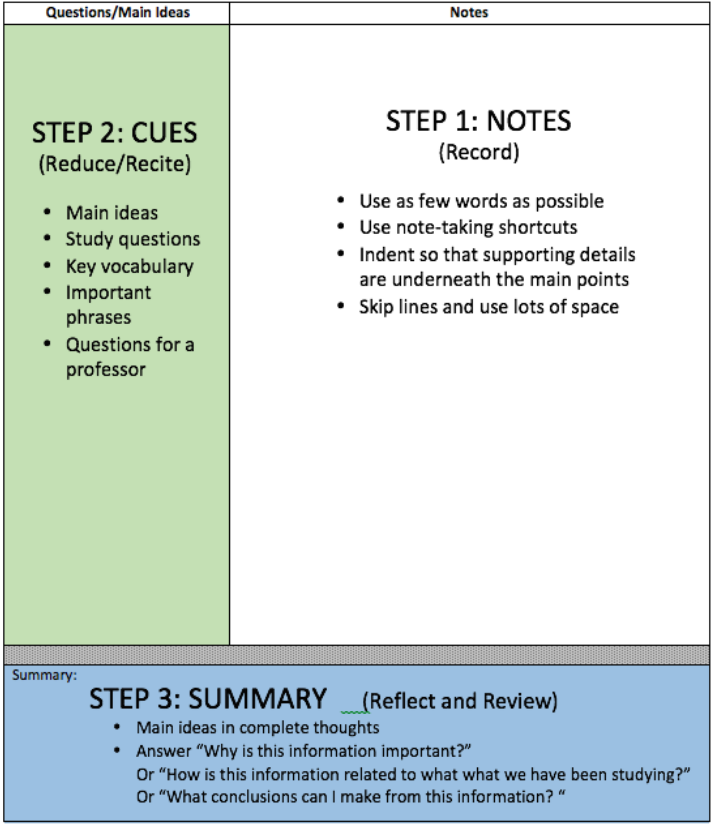
\includegraphics[scale =0.6]{figures/Note_template.png}
\caption{Note-talking template}
\end{figure}

\pagebreak
 
\end{document}